\documentclass{beamer}

\mode<presentation> {


%\usetheme{Darmstadt}
%\usetheme{Dresden}
    \usetheme{Singapore}
%\usetheme{Szeged}
%\usetheme{Warsaw}

%\usecolortheme{albatross}
%\usecolortheme{beaver}
%\usecolortheme{beetle}
%\usecolortheme{crane}
%\usecolortheme{dolphin}
%\usecolortheme{dove}
%\usecolortheme{fly}
%\usecolortheme{lily}
%\usecolortheme{orchid}
%\usecolortheme{rose}
%\usecolortheme{seagull}
%\usecolortheme{seahorse}
%\usecolortheme{whale}
%\usecolortheme{wolverine}

%\setbeamertemplate{footline} % To remove the footer line in all slides uncomment this line
%\setbeamertemplate{footline}[page number] % To replace the footer line in all slides with a simple slide count uncomment this line

%\setbeamertemplate{navigation symbols}{} % To remove the navigation symbols from the bottom of all slides uncomment this line
}


\usepackage{booktabs} % Allows the use of \toprule, \midrule and \bottomrule in tables
\usepackage{hyperref}

\usepackage{graphicx} % Allows including images
\graphicspath{ {images/} }
\usepackage{xcolor}




\AtBeginSection[]{
	\begin{frame}
		\vfill
		\centering
		\begin{beamercolorbox}[sep=8pt,center,shadow=true,rounded=true]{title}
			\usebeamerfont{title}\insertsectionhead\par%
		\end{beamercolorbox}
		\vfill
	\end{frame}
}



%----------------------------------------------------------------------------------------
%	TITLE PAGE
%----------------------------------------------------------------------------------------

\title[MARL]{Multiagent Reinforcement Learning:
Rollout and Policy Iteration
    (Bertsekas, 2020)}
\author{Mikalai Korbit} % Your name

\institute[IMT] % Your institution as it will appear on the bottom of every slide, may be shorthand to save space
{
    IMT School for Advanced Studies Lucca %\\ % Your institution for the title page
%\medskip
%\textit{todo@outlook.com} % Your email address
}
\date{\today} % Date, can be changed to a custom date

\begin{document}

    \begin{frame}
        \titlepage % Print the title page as the first slide
    \end{frame}

    \begin{frame}
        \frametitle{Outline} % Table of contents slide, comment this block out to remove it
        \tableofcontents % Throughout your presentation, if you choose to use \section{} and \subsection{} commands, these will automatically be printed on this slide as an overview of your presentation
    \end{frame}


%----------------------------------------------------------------------------------------
%	PRESENTATION SLIDES
%----------------------------------------------------------------------------------------


%------------------------------------------------


    \section{MARL Overview}
%------------------------------------------------




    \begin{frame}
        \frametitle{Motivation}

        \begin{block}{Multi-agent systems are ubiquitous}
            Eg. fleet of drones, factory robots, self-driving cars.
        \end{block}

        \begin{block}{Recent advances in RL applications}
            Eg. AlphaGo/AlphaZero, playing Starcraft, robotic control.
        \end{block}

        \begin{block}{Utilize modern computer architecture and software frameworks}
            Eg. cloud computing, stacks of graphics cards, TPUs;
            PyTorch, OpenAI gyms.
        \end{block}

        \begin{block}{Benefits of modeling a problem as MARL}
            Scalability, robustness, faster learning through experience sharing,
            parallel computation.
        \end{block}

    \end{frame}



%------------------------------------------------


    \begin{frame}
        \frametitle{Multi-Agent Reinforcement Learning Problem}
        Inherits Reinforcement Learning characteristics:
        \begin{itemize}
            \item Learning how to map situations into actions
            \item Trial-and-error search
            \item Delayed feedback
            \item Trade-off between exploration and exploitation
            \item Sequential decision making
            \item Agent's actions affect the subsequent data it receives
        \end{itemize}

        Adds multi-agent features:
        \begin{itemize}
            \item Actions of one agent influence other agents' rewards
            \item Communication problem
            \item Fully cooperative, fully info sharing (DP) vs. partial info sharing
            \item Curse of dimensionality (more severe than in RL)
        \end{itemize}

    \end{frame}


%------------------------------------------------

\begin{frame}
	\frametitle{``Bertsekas Dictionary''}
	
	Aligns optimal control definitions with the RL-world:
	\begin{itemize}
		\item Maximize value $\rightarrow$ minimize cost		
		\item Agent $\rightarrow$ Decision maker or controller
		\item Action $\rightarrow$ Decision or control
		\item Environment  $\rightarrow$ Dynamic system
		\item Learning $\rightarrow$ Solving a DP-related problem using simulation
		\item Self-learning (self-play) $\rightarrow$ Solving a DP problem using simulation-based policy iteration
		\item Planning vs Learning distinction $\rightarrow$ Solving a DP problem with model-based vs model-free simulation	
	\end{itemize}
	
\end{frame}


%------------------------------------------------


    \begin{frame}
        \frametitle{Multi-Agent MDP}

        \begin{figure}
            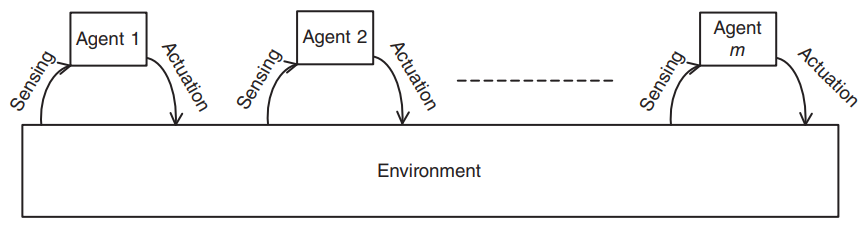
\includegraphics[scale=0.65]{1a_marl}
            \caption{MARL Problem. Source: Sadhu, Konar (2020)}
        \end{figure}

        \begin{itemize}
            \item All agents see the global state $s$
            \item Individual actions: $u^{a} \in U$
            \item State transitions: $P\left(s^{\prime} \mid s, \mathbf{u}\right): S \times \mathbf{U} \times S \rightarrow[0,1]$
            \item Shared team reward: $S \times \mathbf{U} \rightarrow \mathbb{R}$ 
            
            
        \end{itemize}

    \end{frame}


%------------------------------------------------


    \begin{frame}
        \frametitle{Taxonomy}

        \begin{block}{Cooperative}
            \begin{itemize}
                \item The goal of cooperative agents is to achieve a common objective
                \item Coordination problem
            \end{itemize}
        \end{block}

        \begin{block}{Competitive}
            \begin{itemize}
                \item Zero-sum games (eg. chess, tic-tac-toe)
                \item Minimax equilibria
            \end{itemize}
        \end{block}

        \begin{block}{Mixed}
            \begin{itemize}
                \item  General-sum games (win-win, lose-lose scenarios;
                eg. pollution model, ``what movie to watch?'')
                \item  Nash equilibria
            \end{itemize}
        \end{block}

    \end{frame}

%------------------------------------------------


    \begin{frame}
        \frametitle{Algorithms for Cooperative MARL}

        \begin{block}{Static games}
            \begin{itemize}
                \item JAL (Joint Action Learners)
                \item FMQ (Frequency Maximum Q-value)
            \end{itemize}

        \end{block}

        \begin{block}{Dynamic games}
            \begin{itemize}
                \item Team-Q
                \item Distributed-Q
                \item OAL (Optimal Adaptive Learning)
                \item SCQL (Sparse Cooperative Q-learning )
                \item SQL (Sequential Q-learning)
                \item FMRQ (Frequency of the maximum reward Q-learning)
            \end{itemize}
        \end{block}

    \end{frame}



























%------------------------------------------------


    \section{Multiagent Rollout}
%------------------------------------------------


    \begin{frame}
	\frametitle{Key Ideas}
	
	
        \begin{block}{Deal with the exponential increase in the action space}
	$\rightarrow$ Introduce a form of sequential
	agent-by-agent one-step lookahead minimization --
	\textit{multiagent rollout}
	
\end{block}

\begin{block}{Compute the agent actions in parallel}
	$\rightarrow$ Decouple sequential 
	agent-by-agent computation with \textit{precomputed
		signaling policy} that embodies agent coordination
\end{block}	
	
	

	\end{frame}


%------------------------------------------------



    \begin{frame}
        \frametitle{The Setting}
        
        \begin{itemize}
			\item $P2_F$ -- stochastic discrete-time optimal control problem over a finite horizon, with perfect information on the state
			\item Fully cooperative
			\item Tested in Spiders-And-Flies environment
		\end{itemize}
	
	$$x_{k+1}=f_{k}\left(x_{k}, u_{k}, w_{k}\right), \quad k=0,1, \ldots, N-1$$
	
	$$J_{\pi}\left(x_{0}\right)=E\left\{g_{N}\left(x_{N}\right)+\sum_{k=0}^{N-1} g_{k}\left(x_{k}, \mu_{k}\left(x_{k}\right), w_{k}\right)\right\}$$
	
	
    \end{frame}


%------------------------------------------------


    \begin{frame}
	\frametitle{Policy Iteration and Rollout}
	
    \begin{figure}
		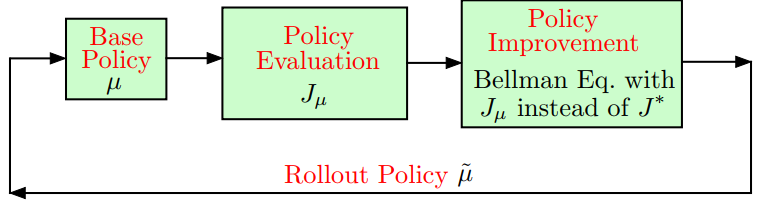
\includegraphics[scale=0.65]{2a_pi}
		\caption{Policy Iteration Algorithm. Source: Bertsekas (2020)}
	\end{figure}
	
	
	\begin{itemize}
		\item Fundamental property: policy improvement
		$$J_{k, \tilde{\pi}}\left(x_{k}\right) \leq J_{k, \pi}\left(x_{k}\right), \quad \forall x_{k}, k$$
		
	\end{itemize}
	
	\end{frame}


%------------------------------------------------


\begin{frame}
	\frametitle{All-at-once Rollout}
	
	\begin{itemize}
		\item Rollout is one-time policy iteration

$$
\begin{aligned}
\tilde{u}_{k} \in \arg \min _{u_{k} \in U_{k}\left(x_{k}\right)} E\left\{g_{k}\left(x_{k}, u_{k}, w_{k}\right) + \right.\\
&\left.+J_{k+1, \pi}\left(f_{k}\left(x_{k}, u_{k}, w_{k}\right)\right)\right\}
\end{aligned}
$$

		\item Rollout is an on-line algorithm and possesses robustness property 
		\item Rollout suffers from dimensionality curse problem when 
		the action space is large (eg. exponential in the number of agents)
		
	\end{itemize}
	
\end{frame}

%------------------------------------------------


\begin{frame}
	\frametitle{One-at-a-time Rollout}
	
    \begin{figure}
	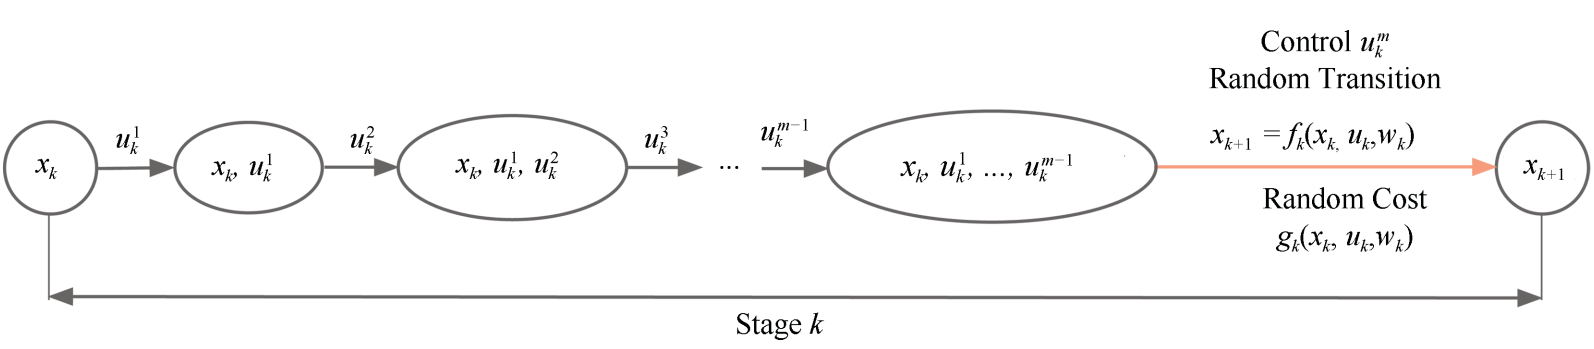
\includegraphics[scale=0.4]{2b}
	\caption{One-at-a-time action selection. Source: Bertsekas (2020)}
	\end{figure}	
	
		
	\begin{enumerate}
		\item Break down $u_k$ into the sequence of $m$ actions: 
		$u^1_k, u^2_k, ..., u^m_k$
		
		\item Introduce artificial states $\left(x_{k}, u_{k}^{1}\right),\left(x_{k}, u_{k}^{1}, u_{k}^{2}\right), \ldots,\left(x_{k}, u_{k}^{1}, \ldots, u_{k}^{m-1}\right)$
		\item $u^m_k$ marks the transition to the new state 
		$x_{k+1}=f(x_k, u_k, w_k)$ incurring cost $g_k(x_k, u_k, w_k)$
	\end{enumerate}


	
\end{frame}


%------------------------------------------------

    \begin{frame}
	\frametitle{Benefits of the Multiagent Rollout Algorithm}
	
			Past controls determined by
		the rollout policy, and the future controls determined by
		the base policy!
	
	
	
	\begin{itemize}
		\item Reducing the action space by increasing the state space. Reasonable since Q-factor minimization is performed for just
		one state at each stage. 	
		
		\item We reduce the computation complexity 
		from $O(q^m)$ to $O(qm)$, $q=|U|$
	\end{itemize}
	
	
	\end{frame}

%------------------------------------------------

\begin{frame}
	\frametitle{Policy Improvement for Multiagent Rollout}
	
	Claim: multi-agent rollout performs about as well as
	standard rollout (all-at-once)
	
	Proof: TODO 	
	
	
	
\end{frame}

%------------------------------------------------
    \begin{frame}
    	
	\frametitle{Ordering of Agents}
	
	
	
	\begin{itemize}
		\item Instead of random order, at each step
	\end{itemize}
	
	
	\end{frame}













%------------------------------------------------
    \section{Extensions}
%------------------------------------------------

    \begin{frame}
        \frametitle{Reinforcement Learning Problem}
        \begin{itemize}
            \item Learning how to map situations to actions
            \item Trial-and-error search
            \item Delayed feedback
            \item Trade-off between exploration and exploitation
            \item Sequential decision making
            \item Agent's actions affect the subsequent data it receives
        \end{itemize}
    \end{frame}


%------------------------------------------------


    \section{Conclusion}

    \begin{frame}
        \frametitle{Conclusion}
        \begin{itemize}
            \item RL methods can be applicable to
            a wide variety of problems

            \item Out-of-the-box models work but
            require fine-tuning and take
            longer to converge

            \item Simple methods like state discretization
            are worth exploring when training speed and
            solution complexity are of the essence

        \end{itemize}
    \end{frame}


    \begin{frame}
        \frametitle{References}
        \footnotesize{
            \begin{thebibliography}{10}

                \bibitem{bert20}\label{bert20}
                Dimitri Bertsekas -- Multiagent Reinforcement Learning: Rollout and Policy Iteration (2020). Web:
                \url{https://web.mit.edu/dimitrib/www/Multiagent_Sinica_2020.pdf}

                \bibitem{whiteson20}\label{whiteson20}
                Shimon Whiteson -- Factored Value Functions for Cooperative Multi-Agent Reinforcement Learning (2020) [Seminar].


                \bibitem{sadhu20}\label{sadhu20}
                Arup Kumar Sadhu, Amit Konar --
                Multi-Agent Coordination,
                A Reinforcement Learning Approach (2020).


            \end{thebibliography}
        }
    \end{frame}

%------------------------------------------------

    \begin{frame}

        \begin{center}
            \Huge Thanks for
            \\
            your attention!
        \end{center}

    \end{frame}

%----------------------------------------------------------------------------------------

\end{document}